\chapter{Evaluation}
% take a step back and put your results from 4 into context. 
This chapter critically examines the machine learning models conceived and partially implemented in the previous chapter.
Table~\ref*{tab:evaluation_criteria} shows an overview of the evaluated criteria. These are structured according to the Goal-Question-Metric approach Mean Absolute Error (MAE) how far the predictions are from the actual output.

\captionsetup{margin={5pt,5pt}}

\begin{table}[H]
    \begin{tcolorbox}[arc=0pt,boxrule=0.5pt]
        \sisetup{group-minimum-digits = 4}
        \centering
        \caption{Overview of the goals, questions and metrics for the evaluation of artifacts following the \ac{GQM} approach.}
        \label{tab:evaluation_criteria_2}
        {\renewcommand{\arraystretch}{1}
            \begin{tabular}{p{2.5cm}p{6cm}p{3cm}}
                \toprule
                \thead{\textbf{Goal}}         & \thead{\textbf{Question}}                                                                                       & \thead{\textbf{Metric}}                              \\

                \hdashline
                \textbf{Appropriatness}       & How well does the model type fit the current task?                                                              & Prerequisites for model type                         \\

                \hdashline
                \textbf{Correctness}          & Ability of the model to perform the current task measured on the development dataset and the runtime dataset    &
                Precision, Recall, F-score                                                                                                                                                                             \\
                \hdashline
                \textbf{Relevance}            & Does the model achieve a good bias-variance tradeoff? Which means neither overfitting or unterfitting the data. & Variance of cross-validation and fit                 \\

                \hdashline
                \textbf{Robustness}           & Ability of the model to outliers, noise and other data quality issues                                           & Equalized Loss of Accuracy (ELA)                     \\

                \hdashline
                \textbf{Stability}            & Does the artifact generate repeatable results when trained on different data?                                   & Leave-one-out-cross validation stability             \\

                \hdashline
                \textbf{Interpretability}     & How well can the model be explained?                                                                            & Complexity measures (e.g., no. of parameters, depth) \\

                \hdashline
                \textbf{Resource utilization} & How much resources are required to train and run the model?                                                     & Training time, runtime, storage space                \\
                \bottomrule
            \end{tabular}
        } % renew command 
    \end{tcolorbox}
\end{table}

\section{DP1: Appropriateness}
% How well does the model type fit the current task?
% Prerequisites for model type


\section{DP2: Correctness}
% Ability of the model to perform the current task measured on the development dataset and the runtime dataset
The model must be able to perform well on the selected task.
To measure the correctness of the model, the metrics MAE, MSE and RMSE are used.
In the formulas \ref{eq:mae}, \ref{eq:mse} and \ref{eq:rmse} the variable $e_i$ is the prediction error which is the difference between the predicted value by the model the actual value.
$y_i$ is the actual value and $n$ is the number of samples in the testing data set.

\paragraph*{Mean Absolute Error (MAE)}

\begin{equation}
    \label{eq:mae}
    MAE = \frac{1}{n} \sum_{i=1}^{n} |e_i|
\end{equation}

\paragraph*{Mean Squared Error (MSE)}

\begin{equation}
    \label{eq:mse}
    MSE = \frac{1}{n} \sum_{i=1}^{n} e^2
\end{equation}

\paragraph*{Root Mean Squared Error (RMSE)}

\begin{equation}
    \label{eq:rmse}
    RMSE = \sqrt{MSE}
\end{equation}

% What are the differences between the metrics?
% -> Copilot
"The mean absolute error (MAE) and mean squared error (MSE) are the most commonly used metrics for
evaluating the performance of regression models. The MAE is the average of the absolute differences between
the predicted and actual values. The MSE is the average of the squared differences between the predicted and
actual values. The MSE is more sensitive to outliers than the MAE. The RMSE is the square root of the MSE.
The RMSE is the most popular metric for evaluating the performance of regression models. The RMSE is
interpretable in the same units as the response variable. The RMSE is more sensitive to outliers than the MAE."


\begin{figure}[H]
    \centering
    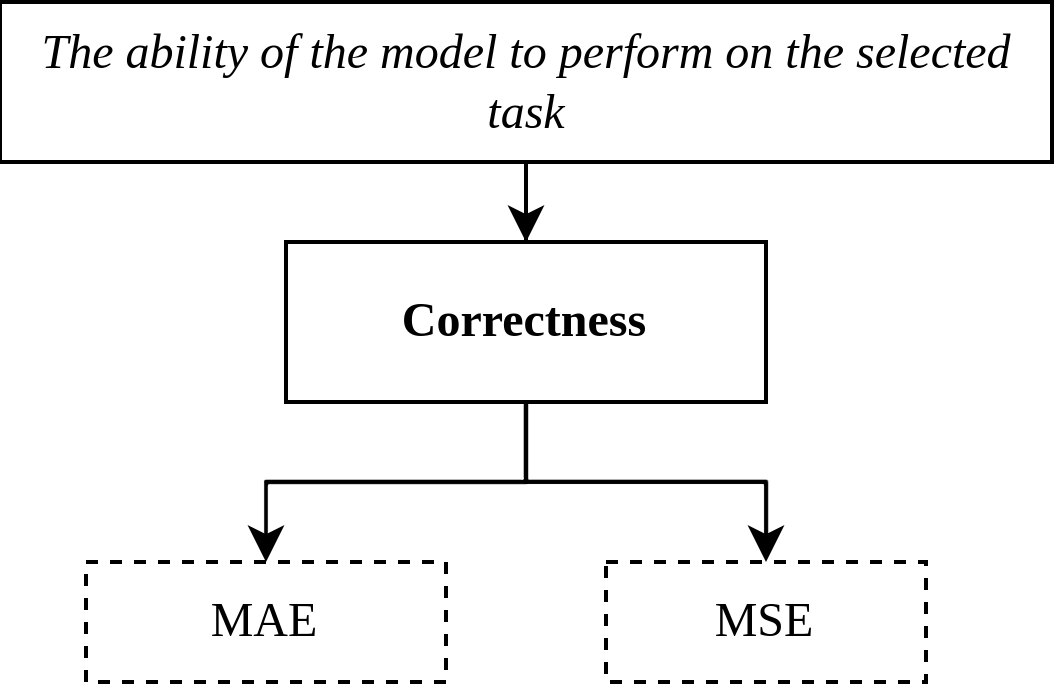
\includegraphics[width=0.6\textwidth]{goal_hierarchie_correctness}
    \caption{Relative feature importance}
    \label{fig:goal_hierarchie_correctness}
\end{figure}


\subsection{Overview of the used machine learning models and their metrics}

% Table wit hall used machine learning models and their metrics
\begin{table}[H]
    \begin{tcolorbox}[arc=0pt,boxrule=0.5pt]
        \sisetup{group-minimum-digits = 4}
        \centering
        \caption{Overview of the used machine learning models and their metrics.}
        \label{tab:ml_models}
        \begin{tabular}{llll}
            \toprule
            \thead{\textbf{Model Name}}        & \thead{\textbf{MAE}}  
                                               & \thead{\textbf{MSE}}
                                               & \thead{\textbf{RMSE}}                              
                                               & \thead{\textbf{R}} \\
            \toprule
            \textbf{Random Forest}             & 0.15                  & 0.03                 & 0.18 & R\\
            \hdashline
            \textbf{Boosting}                  & 0.27                  & 0.07                 & 0.26 & R\\
            \hdashline
            \textbf{Linear Regression}         & 0.27                  & 0.07                 & 0.26 & R\\
            \hdashline
            \textbf{Support Vector Regression} & 0.27                  & 0.07                 & 0.26 & R\\
            \hdashline
        \end{tabular}
    \end{tcolorbox}
\end{table}

% How did baig et al. do it?
% -> MAE, MSE, RMSE 2

% I should cross validation as well to measure genelization performance of each model as well as the stability of the model. 

\begin{figure}[H]
    \centering
    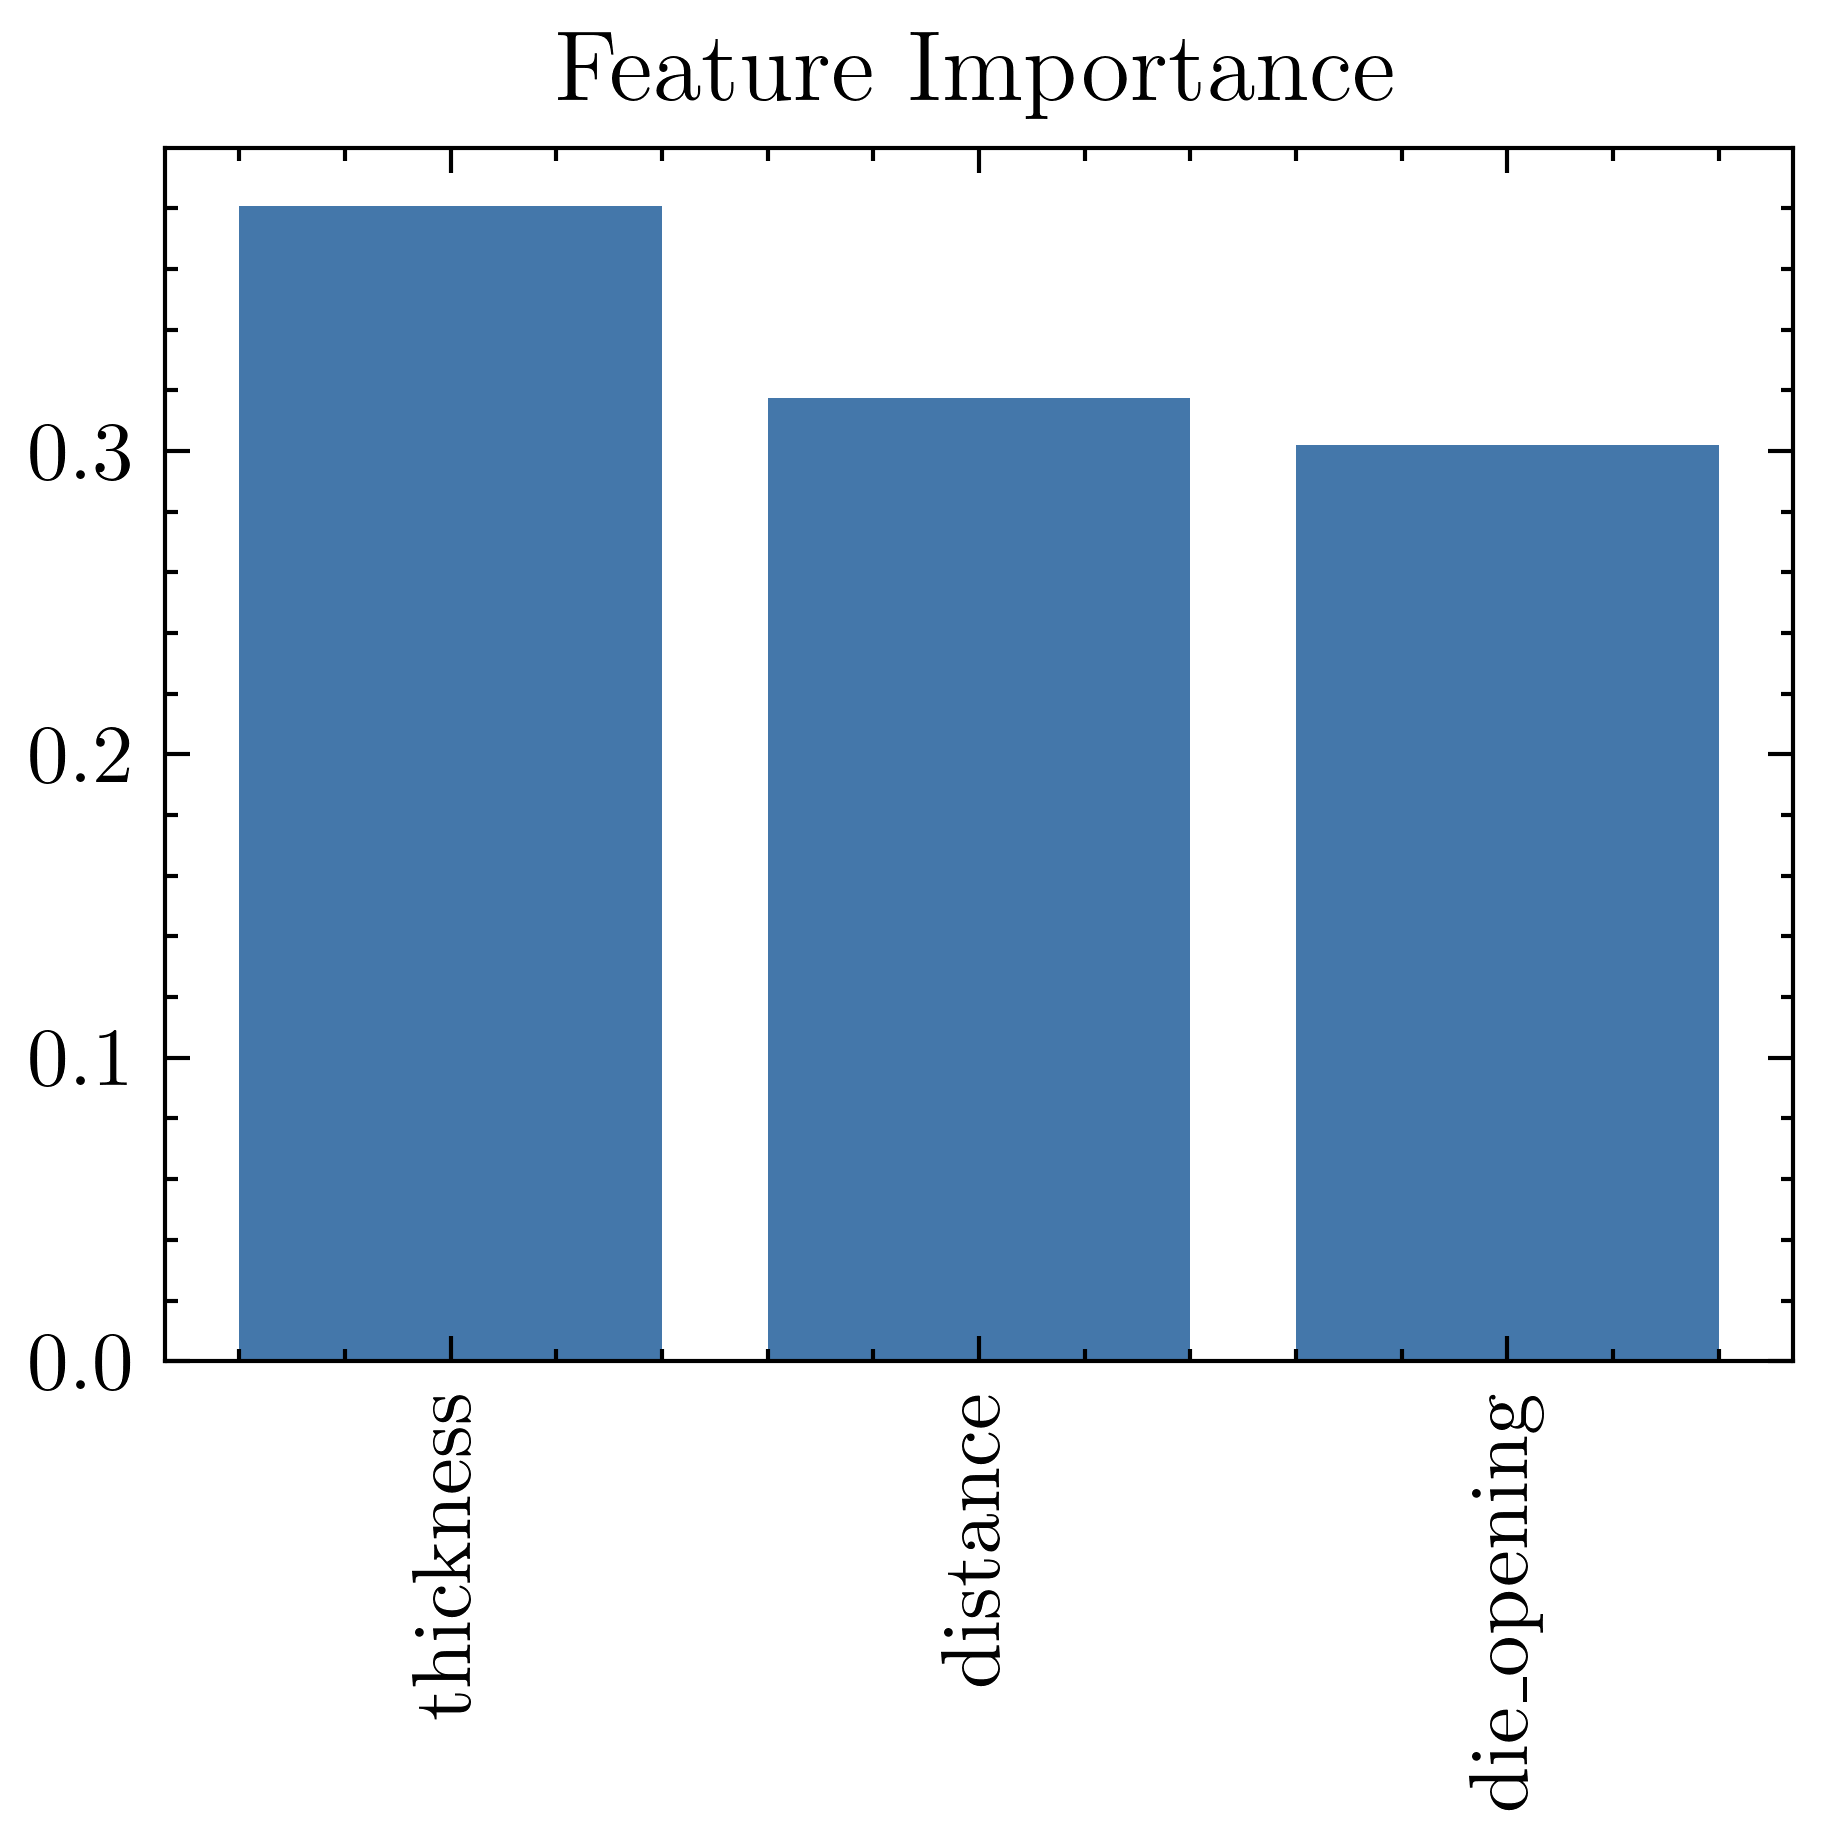
\includegraphics[width=0.6\textwidth]{Random_Forest_Regression_importances}
    \caption{Relative feature importance}
    \label{fig:rf_feature_importance}
\end{figure}

In further experiments boosting was used with the goal of predicting the target vector more precise. A \ac{mse} of 0.27 and \ac{rmse} of 0.52 as achieved and therefore no better performance to the default random forest.


\subsection{Random Forest}
With 100 estimators in \ac{RF} a \ac{mse} of 0.15 and \ac{rmse} 0.39 was achieved.
Figure~\ref{fig:rf_feature_importance} compares and visualizes the relative importance of the features used for training the model.
As shown, the thickness is the most important feature followed by distance and die open. The results show, that all three featured are relevant for the outcome and so no feature can be removed from the dataset to get a better performance of the model.



\section{Relevance}
% Does the model achieve a good bias-variance tradeoff? Which means neither overfitting or unterfitting the data.

% Variance of cross-validation and fit
% -> Fit -> R2


\section{Robustness}
% Ability of the model to outliers, noise and other data quality issues
% Variance of cross-validation, fit

% Equalized Loss of Accuracy (ELA) 

To measure the robustness of the model, the following metrics are used:

\paragraph*{Equalized Loss of Accuracy (ELA)}

\begin{equation}
    \label{eq:ela}
    ELA = \frac{1}{n} \sum_{i=1}^{n} \frac{1}{\hat{y}_i} |y_i - \hat{y}_i|
\end{equation}



\section{Stability}
% Does the artifact generate repeatable results when trained on different data?
% Leave-one-out cross-validation

To measure the stability of the model, the following metrics are used:

\paragraph*{Leave-one-out cross-validation}

\begin{equation}
    \label{eq:loo}
    LOO = \frac{1}{n} \sum_{i=1}^{n} \frac{1}{\hat{y}_i} |y_i - \hat{y}_i|
\end{equation}


\section{Interpretability}
% How well can the model be explained?
% Complexity measures (e.g., no. of parameters, depth)

To measure the interpretability of the model, the following metrics are used:

% From Copilot
\paragraph*{Complexity measures}

\begin{equation}
    \label{eq:complexity}
    Complexity = \frac{1}{n} \sum_{i=1}^{n} \frac{1}{\hat{y}_i} |y_i - \hat{y}_i|
\end{equation}

\section{Resource utilization}
% How much resources are required to train and run the model?
% Training time, runtime, storage space

To measure the resource utilization of the model, the following metrics are used:

% From Copilot
\paragraph*{Training time}

\begin{equation}i
    \label{eq:training_time}
    Training Time = \frac{1}{n} \sum_{i=1}^{n} \frac{1}{\hat{y}_i} |y_i - \hat{y}_i|
\end{equation}

\paragraph*{Runtime}

\begin{equation}
    \label{eq:runtime}
    Runtime = \frac{1}{n} \sum_{i=1}^{n} \frac{1}{\hat{y}_i} |y_i - \hat{y}_i|
\end{equation}

\paragraph*{Storage space}

\begin{equation}
    \label{eq:storage_space}
    Storage Space = \frac{1}{n} \sum_{i=1}^{n} \frac{1}{\hat{y}_i} |y_i - \hat{y}_i|
\end{equation}

\section{Summary}
Using the evaluation metrics described in the previous sections, the following results were achieved.
